\renewcommand{\theequation}{\theenumi}
\begin{enumerate}[label=\arabic*.,ref=\thesubsection.\theenumi]
\numberwithin{equation}{enumi}
\item Find the remainder when $x^3+3x^2+3x+1$ is divided by 
\begin{enumerate}
\item $x+1$
\item $x-\frac{1}{2}$
\item $x$
\item $x+\pi$
\item $5+2x$
\end{enumerate}
%
\item Check whether $7+3x$ is a factor of $3x^3+7x$.
%
\item Determine which of the following polynomials has $(x+1)$ as a factor:
%
\begin{enumerate}
\item $x^3+x^2+x+1$
\item $x^4+x^3+x^2+x+1$
\item $x^4+3x^3+3x^2+x+1$
\item $x^3-x^2-\brak{2+\sqrt{2}}+\sqrt{2}$.
\end{enumerate}
%
\item Determine whether $g(x)$ is a factor of $p(x)$ in each of the following cases:
%
\begin{enumerate}
\item $p(x) = 2x^3+x^2-2x-1, g(x) = x+1$
\item $p(x) = x^3+3x^2+3x+1, g(x) = x+2$
\item $p(x) = x^4-4x^2+x+6, g(x) = x-3$
\end{enumerate}
%
\item  Factorise : 
\begin{enumerate}
\item $x^3 – 2x^2 – x + 2 $
\item $x^3– 3x^2 – 9x – 5 $
 \item $x^3+ 13x^2 + 32x + 20 $
\item $2y^3+ y^2– 2y – 1$
\end{enumerate}
\item Find the roots of the following equations:
\begin{enumerate}
\item  $x - \frac{1}{x} = 3, x \ne =0 $
\item  $ \frac{1}{x+4} - \frac{1}{x-7} = \frac{11}{30}, x\ne =-4, 7 $
\end{enumerate}
%
\item Find the slope of the tangent to the curve $y = 3x^4-4x$ at $x=4$.
\item Find the slope of the tangent to curve $y = x^3-3x+2$ at the point whose 
x-coordinate is 2.
\item Find the slope of the tangent to the curve $y = x^3-3x+2 $ at the point whose x-coordinate is 3.
\item Find the slope of the normal to the curve 
$
\vec{x} = a \myvec{\cos^3\theta \\ \sin^{3}\theta}
$
at $\theta = \frac{\pi}{4}$.
\item Find the slope of the normal to the curve 
$
\vec{x} =  \myvec{1-a\sin\theta \\ b\cos^{2}\theta}
$
at $\theta = \frac{\pi}{2}$.
\item Find points at which the tangent to the curve $y = x^3-3x^2-9x+7$ is parallel to th x-axis.
\item Find the point on the curve $y = x^3– 11x + 5$
at which the tangent is $\myvec{1 & -1}\vec{x} =  11$.
\item Find the equations of all lines having slope 0 which are tangent to the curve 
$
y = \frac{1}{x^2-2x+3}
$.
\item Find the equations of the tangent and normal to the given curves at the indicated points: 
%
\begin{enumerate}
\item
$
y= x^4 - 6x^3+13x^2-10x+5
$
at \myvec{0\\5}.
\item
$
y = x^4 - 6x^3+13x^2-10x+5
$
at \myvec{1\\3}.
\item
$
y = x^3
$
at \myvec{1\\1}.
\end{enumerate}
%
\item Show that the tangents to the curve $y = 7x^3 + 11$ at the points where $x = 2$ and $x = -2$ are parallel.
\item Find the points on the curve $y = x^3$  at which the slope of the tangent is equal to the y-coordinate of the point.
\item For the curve $y = 4x^3 – 2x^5$ find all the points at which the tangent passes through the origin.
\item Find the equation of the normal at the point $\myvec{am^2 \\ am^3}$  for the curve $ay^2 = x^3$
\item Find the equation of the normals to the curve $y = x^3+2x+6$ which are parallel to the line $\myvec{1 & 14} + 4 = 0$.
\item Find the slope of the normal to the curve $y = 2x^2 + 3 \sin x$ at $x = 0$.
%
Show that the normal at any point $\theta$ to the curve $\vec{x} = \myvec{a \cos\theta + a \theta \sin\theta\\  a \sin\theta – a\theta \cos\theta}$ is at a constant distance from the origin.
%
\item Find the slope of the tangent to the curve $\vec{x} = \myvec{t^2+3t-8 \\ 2t^2-2t-5}$
at the point $\myvec{2\\-1}$.
\item Find the points on the curve $9y^2 = x^3$, where the normal to the curve makes equal intercepts with the axes.
\item Find the area under $y = x^4, x = 1, x = 5$ and x-axis.
%
\item Find the area bounded by the curve $y = x^3, x =-2, x = 1$ and the x-axis.
\item Find the area bounded by the curve $y = x \abs{x}, x = -1, x = 1$ and the x-axis.
\item Find the area bounded by the y-axis, $y = \cos x$ and $y = \sin x$ when $0 \le x \le \frac{\pi}{2}$.\item Show that the function given by $f(x) = 3x+17$  is increasing on $\vec{R}$.
\item Show that the function given by $f(x) = e^{2x}$  is increasing on $\vec{R}$.
%
%
\item Show that the function given by 
\begin{align}
f(x)  = \sin x
\end{align}
%
is 
\begin{enumerate}
\item increasing in $\brak{0,\frac{\pi}{2}}$
\item decreasing in $\brak{\frac{\pi}{2}, \pi}$
\end{enumerate}
%
%
\item Find the intervals in which the function given by 
\begin{align}
f(x)  = 2x^3-3x^2 - 36x +7
\end{align}
%
is 
\begin{enumerate}
\item increasing
\item decreasing.
\end{enumerate}
%
\item Find the intervals in which the following functions are strictly increasing or decreasing
%
\begin{enumerate}
\item $\brak{x+1}^3\brak{x-3}^3$
\item $-2x^3-9x^2-12x+1$
\end{enumerate}
%
\item Show that 
%
\begin{align}
y = \log \brak{1+x}-\frac{2x}{2+x}, x > -1,
\end{align}
%
is an increasing function of $x$ throughout its domain.
%
\item Find the values of $x$ for which $y = x\brak{x-2}^2$ is an increasing function.
%
\item Prove that
%
\begin{align}
y = \frac{4\sin \theta}{2+\cos \theta} - \theta
\end{align}
%
is an incresing function of $\theta$ in $\sbrak{0,\frac{\pi}{2}}$.
\item Prove that the logarithmic function is increasing on $\brak{0, \infty}$.
\item Which of the following functions are decreasing on $\sbrak{0,\frac{\pi}{2}}$?
%
\begin{enumerate}
\item $\cos x$
\item $\cos 2x$
\item $\cos 3x$
\item $\tan x$
\end{enumerate}
%
\item Find the intervals on which 
%
\begin{align}
f(x) = x^{100}+\sin x -1
\end{align}
%
is decreasing.
\item Let $I$ be any interval disjoint from $\sbrak{1,-1}$.  Prove that the function $f$ given by $f(x) = x +\frac{1}{x}$ is increasing on $I$.
\item Prove that the function $f$ given by $f(x) = \log \sin x$ is increasing on $\brak{0,\frac{\pi}{2}}$ and decreasing on $\brak{\frac{\pi}{2}, \pi}$.
\item Prove that the function $f$ given by $f(x) = \log \abs{\cos x}$ is decreasing on $\brak{0,\frac{\pi}{2}}$ and increasing on $\brak{\frac{3\pi}{2}, 2\pi}$.
\item Prove that the function given by $f(x) = x^3-3x^2+3x-100$ is increasing in $\vec{R}$.
\item Find the interval(s) in which $f(x) = x^2e^{-x}$ is increasing.
\item Find the maximum and minimum values, if any, of $g(x) = x^3+1$.
%
\item Find the maximum and minimum values, if any of
the following functions given by 
%
\begin{enumerate}
\item $h(x) = \sin\brak{2x} + 5$
\item $f(x) = \abs{\sin\brak{4x} + 3}$
\end{enumerate}
%
\item Find the local maximum and minima, if any, of
the following functions.  Find also the  local maximum and local minimum values, as the case may be
%
\begin{enumerate}
\item $g(x) = x^3-3x$
\item $h(x) = \sin x +\cos x, x \in \brak{0,\frac{\pi}{2}}$
\item $f(x) = \sin x -\cos x, x \in \brak{0,2\pi}$
\item $f(x) = x^3-6x^2+9x+15$
\item $g(x) = \frac{x}{2} + \frac{2}{x}, x > 0$
\item $g(x) = \frac{1}{x^2+2}$
\item $f(x) = x\sqrt{1-x}, 0 < x < 1$.
\end{enumerate}
%
\item Prove that the following functions do not have maxima or minima:
%
\begin{enumerate}
\item $f(x) = e^x$
\item $g(x) = \log x$
\item $h(x) = x^3+x^2+x+1$
\end{enumerate}
\item Find the absolute maximum and absoute minimum value of the following functions in the given intervals
%
\begin{enumerate}
\item $f(x) = x^3, x \in \brak{-2,2}$
\item $f(x) = \sin x + \cos x,  x \in \brak{0,\pi}$.
\end{enumerate}
%
\item Find both the maximum value and the minimum value of 
\begin{align}
3x^4-8x^3+12x^2-48x+25, x \in \sbrak{0,3}.
\end{align}
%
\item At what points in the interval $\sbrak{0,2\pi}$, does the function $\sin 2x$ attain its maximum value?
\item What is the maximum value of the function $\sin x + \cos x$?
\item Find the maximum value of $2x^3-24x+107$ in the interval $\sbrak{1,3}$.  Find the maximum value of the same function in $\sbrak{-3,1}$.
\item It is given that at $x=1$, the function $x^4-62x^2 + ax+9$ attains its maximum value on the interval $\sbrak{0,2}$.  Find the value of $a$.
\item Find the maximum and minimum values of $x + \sin 2x$ on $\sbrak{0, 2\pi}$.
\item For all real values of x, the minimum value of
\begin{align}
\frac{1-x+x^2}{1+x+x^2}.
\end{align}
%
\item Find the maximum value of 
\begin{align}
\sbrak{x\brak{x-1}}^{\frac{1}{3}}.
\end{align}
\item Using differentials, find the approximate value of each of the following
%
\begin{enumerate}
\item $\brak{\frac{17}{81}}^{\frac{1}{4}}$
\item $\brak{33}^{-\frac{1}{5}}$
\end{enumerate}
%
\item Show that the function given by $f(x) = \frac{\log x}{x}$ has maximum at $x = 3$.
\item Find the intervals in which the function $f$ given by 
%
\begin{align}
f(x)  = \frac{4\sin x-2x - x\cos x}{2+\cos x}
\end{align}
%
is
%
\begin{enumerate}
\item increasing 
\item decreasing 
\end{enumerate}
%
\item Find the interals in which the function $f$ given by 
%
\begin{align}
f(x)  = x^3 + \frac{1}{x^3}, \quad x \ne 0
\end{align}
%
is
\begin{enumerate}
\item increasing 
\item decreasing 
\end{enumerate}
%
\item Find the absolute maximum and minimum values of the function $f$ given by 
%
\begin{align}
f(x)  = \cos^2 x + \sin x , \quad x \in \sbrak{0,\pi}
\end{align}
%
\item Find the points at which the function $f$ given by 
%
\begin{align}
f(x)  = \brak{x-2}^4\brak{x+1}^3
\end{align}
%
has
\begin{enumerate}
\item local maxima
\item local minima
\item point of inflexion
\end{enumerate}
%
\item Examine the following functions for continuity.
%
\begin{enumerate}
\item $f(x) = \frac{1}{x-5}$
\item $f(x) = \frac{x^2-25}{x+5}, x \ne -5$
\end{enumerate}
%
\item Prove that the function $f(x) = x^n$ is continuous at $x = n$, where $n$ is a positive integer.
%
\begin{enumerate}
\item 
$
\begin{alignedat}[t]{2}
f(x)=
\begin{cases}
x^3-3, & x \le 2,
\\
x^2+1, & x > 2
\end{cases}
\end{alignedat}
$
\item 
$
\begin{alignedat}[t]{2}
f(x)=
\begin{cases}
x^10-1, & x \le 1,
\\
x^2, & x > 1
\end{cases}
\end{alignedat}
$
\end{enumerate}
%
\item Discuss the continuity of the following functions:
%
\begin{enumerate}
\item 
$
\begin{alignedat}[t]{2}
f(x)= \sin x + \cos x
\end{alignedat}
$
\item 
$
\begin{alignedat}[t]{2}
f(x)= \sin x - \cos x
\end{alignedat}
$
\item 
$
\begin{alignedat}[t]{2}
f(x)= \sin x \cos x
\end{alignedat}
$
\end{enumerate}
\item Discuss the continuity of the cosine, cosecant, secant and cotangent functions.
\item Find all points of discontinuity of $f$, where 
\begin{align}
f(x)=
\begin{cases}
\frac{\sin x}{x}, & x < 0,
\\
x+1, & x \ge 0
\end{cases}
\end{align}
\item Determine if 
\begin{align}
f(x)=
\begin{cases}
x^2\sin \brak{\frac{1}{x}}, & x \ne 0,
\\
0, & x = 0
\end{cases}
\end{align}
%
is a continuous function.
\item Examine the continuity of 
\begin{align}
f(x)=
\begin{cases}
\sin x -\cos x, & x \ne 0,
\\
-1, & x = 0
\end{cases}
\end{align}
%
\item Find values of $k$ so that the following functions are continuous at the points indicated
%
\begin{enumerate}
\item 
$
\begin{alignedat}[t]{2}
\begin{cases}
\frac{k\cos x}{\pi - 2x} & x \ne \frac{\pi}{2},
\\
3, & x = \frac{\pi}{2}
\end{cases},
\end{alignedat}
\quad x = \frac{\pi}{2}
$
\item 
$
\begin{alignedat}[t]{2}
\begin{cases}
kx+1 & x \le \pi, 
\\
\cos x, & x > \pi,
\end{cases}
\quad x = \pi
\end{alignedat}
$
\end{enumerate}
%
\item Show that the function defined by $f(x) = cos (x^2 )$ is a continuous function.
\item  Show that the function defined by $f(x) = \abs{ cos x} $ is a continuous function. 
\item  Examine that $sin \abs{ x}$ is a continuous function. 
\item  Find all the points of discontinuity of $f$ defined by $f(x) = \abs{ x} – \abs{ x + 1 }$.
%%
\item Evaluate the following limits
%
\begin{enumerate}
\item  $\lim_{x\to 4} \frac{4x+3}{x-2}$
\item  $\lim_{x\to -1} \frac{x^10+x^5+1}{x-1}$
\item  $\lim_{x\to 0} \frac{\brak{x+1}^5-1}{x}$
\item  $\lim_{x\to 2} \frac{3x^2-x-10}{x^2-4}$
\item  $\lim_{x\to 3} \frac{x^4-81}{2x^2-5x-3}$
\item  $\lim_{x\to 0} \frac{ax+b}{cx+1}$
\item  $\lim_{z\to 1} \frac{z^{\frac{1}{3}}-1}{z^{\frac{1}{6}}-1}$
\item  $\lim_{x\to 1} \frac{ax^2+bx+3}{cx^2+bx+a}, \quad a+b+c \ne 0$
\item  $\lim_{x\to 2} \frac{\frac{1}{x}+\frac{1}{2}}{x+2}$
\item  $\lim_{x\to 0} \frac{\sin ax}{bx}$
\item  $\lim_{x\to 0} \frac{\sin ax}{\sin bx}, \quad a,b \ne 0$
\item  $\lim_{x\to \pi} \frac{\sin \brak{\pi-x}}{\pi \brak{\pi-x}}, \quad a,b \ne 0$
\item  $\lim_{x\to 0} \frac{\cos x}{\pi -x}$
\item  $\lim_{x\to 0} \frac{\cos 2x-1}{\cos x-1}$
\item  $\lim_{x\to 0} \frac{ax + x\cos x}{b\sin x}$
\item  $\lim_{x\to 0} x\sec x$
\item  $\lim_{x\to 0} \frac{\sin ax + bx}{ax+\sin bx}, \quad a,b, a+b \ne 0$
\item  $\lim_{x\to 0} \csc - \cot x$
\item  $\lim_{x\to \frac{\pi}{2}} \frac{\tan 2x}{x-\frac{\pi}{2}}$
\end{enumerate}
%
\item Find $\lim_{x\to 0} f(x)$ and $\lim_{x\to 1} f(x)$where
\begin{align}
f(x) = 
\begin{cases}
2x+3 & x \le 0
\\
3\brak{x+1}, & x > 0
\end{cases}
\end{align}
%
\item Let $a_1, a_2, \dots a_n$ be fixed real numbers and define a function
\begin{align}
f(x) = \brak{x-a_1}\brak{x-a_2}\dots \brak{x-a_n}
\end{align}
%
What is $\lim_{x\to a_1} f(x)$?  For some $a \ne a_1, a_2, \dots, a_n$, compute $\lim_{x\to a} f(x)$.
%
\item If 
%
\begin{align}
\lim_{x\to 1} \frac{f(x)-2}{x^2-1} = \pi, 
\end{align}
%
evaluate $\lim_{x\to 1} f(x)$.
%
\item If 
%
\begin{align}
f(x) = 
\begin{cases}
mx^2+n & x < 0
\\
nx +m, & 0\le x \le 1
\\
nx^3+m, & x > 1,
\end{cases}
\end{align}
%
for what integers $m$ and $n$ does both  $\lim_{x\to 0} f(x)$ and $\lim_{x\to 1} f(x)$ exist ?
%
%\item Differentiate the following functions with respect to $x$
%%
%\begin{enumerate}
%\item 
%$
%\sin \brak{x^2+5}
%$
%\item 
%$
%\cos \brak{\sin x}
%$
%\item 
%$
% \sin\brak{ax+b}
%$
%\item 
%$
%\sec \brak{\tan \sqrt{x}}
%$
%\item 
%$
%\frac{\sin \brak{ax+b}}{\cos \brak{ cx+d}}
%$
%\item 
%$
%\cos x^3 \sin^2\brak{x^5}
%$
%\item 
%$
%2\sqrt{\cot \brak{x^2}}
%$
%\item 
%$
%\cos\brak{\sqrt{x}}
%$
%\end{enumerate}
%\item Find $\frac{dy}{dx}$ in the following:
%\begin{enumerate}
%\item 
%$
%2x+3y = \sin x
%$
%\item 
%$
%2x+3y = \sin y
%$
%\item 
%$
%ax + by^2 = \cos y
%$
%\item 
%$
%xy+y^2 = \tan x + y
%$
%\item 
%$
%x^3+x^2y+xy^2+y^3 = 81
%$
%\item 
%$
%\sin^2 y + \cos xy = \kappa
%$
%\item 
%$
%\sin ^2 x + \cos ^2 y = 1
%$
%\item 
%$
%y = \sin^{-1}\brak{\frac{2x}{1+x^2}}
%$
%\item 
%$
%y = \tan^{-1}\brak{\frac{3x-x^2}{1-3x^2}}, x \in \brak{-\frac{1}{\sqrt{3}}, \frac{1}{\sqrt{3}}}
%$
%\item 
%$
%y = \cos^{-1}\brak{\frac{1-x^2}{1+x^2}}, 0 < x < 1
%$
%\item 
%$
%y = \sin^{-1}\brak{\frac{1-x^2}{1+x^2}}  < x < 1
%$
%\item 
%$
%y = \cos^{-1}\brak{\frac{2x}{1+x^2}}, - 1 < x < 1
%$
%\item 
%$
%y = \sin^{-1}\brak{2x\sqrt{1-x^2}}, -\frac{1}{\sqrt{2}} < x < \frac{1}{\sqrt{2}}
%$
%\item 
%$
%y = \sec^{-1}\brak{\frac{1}{2x^2-1}}, 0 < x < \frac{1}{\sqrt{2}}
%$
%\end{enumerate}
%\item Differentiate the following w.r.t. $x$:
%\begin{enumerate}
%\item 
%$
%\frac{e^x}{\sin x}
%$
%\item 
%$
%e^{\sin ^{-1} x}
%$
%\item 
%$
%e^{x^3}
%$
%\item 
%$
%\sin \brak{\tan ^{-1}e^{-x}}
%$
%\item 
%$
%\log\brak{\cos e^x}
%$
%\item 
%$
%e^x + e^{x^2}+\dots+e^{x^5}
%$
%\item 
%$
%\sqrt{e^{\sqrt{x}}}, x > 0
%$
%\item 
%$
%\log\brak{\log x}, x > 1
%$
%\item 
%$
%\frac{\cos x}{\log x}, x > 0
%$
%\item 
%$
%\cos \brak{\log x + e^x}, x > 0
%$
%\end{enumerate}
%\item Differentiate the following w.r.t. $x$
%\begin{enumerate}
%\item 
%$
%\cos x \cos 2x \cos 3x
%$
%\item 
%$
%\sqrt{\frac{\brak{x-1}\brak{x-2}}{\brak{x-3}\brak{x-4}\brak{x-5}}}
%$
%\item 
%$
%\brak{\log x}^{\cos x}
%$
%\item 
%$
%x^x - 2^{\sin x}
%$
%\item 
%$
%\brak{x+3}^2\brak{x+4}^3\brak{x+5}^4
%$
%\item 
%$
%\brak{x + \frac{1}{x}}^x+x^{1+\frac{1}{x}}
%$
%\item 
%$
%\brak{\log x}^x + \brak{\sin x}^{\cos x}
%$
%\item 
%$
%\brak{\sin x}^x +\sin^{-1}\sqrt{x}
%$
%\item 
%$
%x^{\sin x} + \brak{\sin x}^{\cos x}
%$
%\item 
%$
%x^{\cos x} + \frac{x^2+1}{x^2-1}
%$
%\item 
%$
%\brak{x \cos x}^x + \brak{x \sin x}^{\frac{1}{x}}
%$
%\item 
%$
%x^{y}+y^x = 1
%$
%\item 
%$
%y^x = x^y
%$
%\item 
%$
%\brak{\cos x}^y = \brak{\cos y}^{x}
%$
%\item
%$
%xy = e^{x-y}
%$
%\end{enumerate}
%\item Find the derivative of the function given by 
%$
%f(x) = \brak{1+x}\brak{1+x^2}\brak{1+x^4}\brak{1+x^8}
%$
%and hence find $f^{\prime} 1$.
%\item Differentiate 
%$
%\brak{x^2-5x+8}\brak{x^3+7x+9}
%$
%in three ways mentioned below:
%\begin{enumerate}
%\item by using product rule
%\item by expanding the product to obtain a single polynomial
%\item by logarithmic differentiation.
%\end{enumerate}
%%
%Do they all give the same answer?
%\item Without eliminating the parameter, find $\frac{dy}{dx}$ in the following
%%
%\begin{enumerate}
%\item
%$
%x = 2at^2, y = at^4
%$
%\item
%$
%x = a\cos\theta, y =b\cos \theta
%$
%\item
%$
%x = \sin t, y =\cos t
%$
%\item
%$
%x = 4t, y = \frac{4}{t}
%$
%\item
%$
%x = \cos \theta - \cos 2\theta, y = \sin \theta  - \sin 2\theta
%$
%\item
%$
%x = a \brak{\theta - \sin \theta}, y = a\brak{1+\cos \theta}
%$
%\item
%$
%x = \frac{\sin ^3 t}{\sqrt{\cos 2t}}, y =\frac{\cos ^3 t}{\sqrt{\cos 2t}}
%$
%\item
%$
%x = a\brak{\cos t + \log \tan \frac{t}{2}} , y = a \sin t
%$
%\item
%$
%x = a\sec \theta , y = b \tan \theta
%$
%\item
%$
%x = a\brak{\cos \theta + \theta \sin \theta}, y = a\brak{\sin \theta - \theta \cos \theta}
%$
%\item If 
%$
%x = \sqrt{a^{\sin^{-1}t}}, y = \sqrt{a^{\cos^{-1}t}}
%$
%\end{enumerate}
%%
%show that $\frac{dy}{dx} = -\frac{y}{x}$.
%%
%\item Find the second order derivatives of the following functions
%\begin{enumerate}
%\item
%$
%x^2+3x+2
%$
%\item
%$
%x^{20}
%$
%\item
%$
%x\cos x
%$
%\item
%$
%\log x
%$
%\item
%$
%x^3\log x
%$
%\item
%$
%x^x\sin 5x
%$
%\item
%$
%e^{6x}\cos 3x
%$
%\item
%$
%\tan ^{-1}x
%$
%\item
%$
%\log \brak{\log x}
%$
%\item
%$
%\sin\brak{\log x}
%$
%
%\end{enumerate}
%%
%\item If $y = 5\cos x - 3 \sin x$, prove that 
%$
%\frac{d^2y}{dx^2} +y = 0
%$
%\item If $y = \cos^{-1}x$, find $\frac{d^2y}{dx^2}$ in terms of $y$.
%\item If 
%$
%y = 3 \cos \brak{\log x} + 4\sin\brak{\log x}, 
%$
%show that 
%$
%x^2y_2+xy_1+y = 0
%$
%\item If 
%$
%y = Ae^{mx} + Be^{nx}, 
%$
%show that 
%$
%y_2 - \brak{m+n}y_1 +mny = 0.
%$
%\item If 
%$
%y = 500e^{7x} + 600 e^{-7x}, 
%$
%show  that 
%$
%y_2 = 49y
%$
%\item If 
%$
%e^y\brak{x+1} = 1,
%$
%show that 
%$
%y_2 = y_1^2
%$
%\item If 
%$
%y = \brak{\tan^{-1}x}^2, 
%$
%show that 
%$
%\brak{x^2+1}y_2+2x\brak{x^2+1}y_1 = 2
%$
%\item If $f: \sbrak{-5,5}\to \vec{R}$ is a differentiable function and if $f^{\prime}(x)$ does not vanish anywhere, then prove that $f(-5) \ne f(5)$.
%\item Verify mean value theorem, if 
%$
%f(x) = x^3-5x^2-3x, x \in \sbrak{a,b}
%$
%where $a = 1, b = 3$.  Find all $c \in \brak{1,3}$ for which $f^{\prime}(c) = 0$
%%
%\item Differentiate the following functions w.r.t x
%%
%\begin{enumerate}
%\item 
%$
%\brak{3x^2-9x+5}^9
%$
%\item 
%$
%\sin^3x+\cos^6x
%$
%\item 
%$
%\brak{5x}^{3\cos2x}
%$
%\item 
%$
%\sin^{-1}\brak{x\sqrt{x}}, \quad 0 \le x \le 1
%$
%\item 
%$
%\frac{\cos^{-1}\frac{x}{2}}{\sqrt{2x+7}}, -2 < x < 2
%$
%\item 
%$
%\cot^{-1}\sbrak{\frac{\sqrt{1+\sin x}+\sqrt{1-\sin x}}{\sqrt{1+\sin x}-\sqrt{1-\sin x}}}, 0 < x < \frac{\pi}{2}
%$
%\item 
%$
%\brak{\log x}^{\log x}, x > 1
%$
%\item 
%$
%\cos\brak{a\cos x + b \sin x}, 
%$
%for some constant $a$ and $b$.
%\item 
%$
%\brak{\sin x - \cos x}^{\sin x - \cos x}, \quad \frac{\pi}{4}, < x < \frac{3\pi}{4}
%$
%\item 
%$
%x^x+x^a+a^x+a^a,
%$
%for some fixed $a > 0$ and $x > 0$.
%\item 
%$
%x^{x^2-3}_+\brak{x-3}^{x^2}, 
%$
%for $x > 3$.
%\end{enumerate}
%\item Find $\frac{dy}{dx}$, if $y = 12\brak{1-\cos t}, x = 10\brak{t-\sin t}, -\frac{\pi}{2} < x < \frac{\pi}{2}$.
%\item Find $\frac{dy}{dx}$, if 
%$
%y = \sin ^{-1}x + \sin^{-1}\sqrt{1-x^2}, \quad 0 < x < 1
%$
%\item If 
%$
%x\sqrt{1+y}+y\sqrt{1+x} = 0,
%$
%for $-1<x<1$, prove that
%%
%\begin{align}
%\frac{dy}{dx} = -\frac{1}{\brak{1+x}^2}
%\end{align}
%\item If
%$
%\cos y = x \cos\brak{a+y}, 
%$
%with 
%$
%\cos a \ne \pm 1,
%$
%prove that 
%$
%\frac{dy}{dx}= \frac{\cos^2\brak{a+y}}{\sin a}
%$
%\item if 
%$
%x = a \brak{\cos t + t\sin t}
%$
%and
%$
%y = a \brak{\sin t - t\cos t }, 
%$
%find $y_2$
%\item If $f(x) =\abs{x}^3$, show that $f^{''}(x)$ exists for all real $x$ and find it.
%\item Using mathematical induction, prove that $\frac{d}{dx}\brak{x^n} = nx^{n-1}$ for all positive integers $n$.
%\item Using the fact that 
%\begin{align}
%\sin\brak{x+y} = \sin x \cos y +\cos x \sin y,
%\end{align}
%%
%show that 
%\begin{align}
%\cos\brak{x+y} = \cos x \cos y -\sin x \sin y
%\end{align}
%\item If 
%\begin{align}
%y = 
%\mydet{
%f(x) & g(x) & h(x)
%\\
%l &m & n
%\\
%a & b & c
%},
%\end{align}
%%
%prove that 
%\begin{align}
%\frac{dy}{dx} = 
%\mydet{
%f^{'}(x) & g^{'}(x) & h^{'}(x)
%\\
%l &m & n
%\\
%a & b & c
%}
%\end{align}
%\item If $y = e^{a\cos^{-1}x}, - 1 \le x \le 1$, show that 
%\begin{align}
%\brak{1-x^2}y_2-xy_1-ay^2 = 0.
%\end{align}
%%
%
%\item Find the derivative of the following functions from the first principle:
%%
%\begin{enumerate}
%\item  $x^3-27$
%\item  $\frac{1}{x^2}$
%\item  $\frac{x+1}{x-1}$
%\end{enumerate}
%%
%\item For the function 
%\begin{align}
%f(x) = \frac{x^100}{100} + \frac{x^99}{99} + \dots + \frac{x^2}{2} + x + 1.
%\end{align}
%%
%prove that $f^{'}(1) = 100f^{'}(0) $.
%%
%\item Find the derivative of 
%\begin{align}
%x^n+ax^{n-1}+a^2x^{n-2}+\dots+a^n
%\end{align}
%%
%for some fixed real number $a$.
%%
%\item For some constans $a$ and $b$, find the derivative of
%%
%\begin{enumerate}
%\item  $\brak{ax^2+b}^2$
%\item  $\frac{x-a}{x-b}$
%\end{enumerate}
%%
%\item Find the derivative of $\frac{x^n-a^n}{x-a}$ for some constant $a$.
%%
%
%\item Find the derivative of 
%%
%\begin{enumerate}
%\item  $2x-\frac{3}{4}$
%\item  $\brak{5x^3+3x-1}\brak{x-1}$
%\item  $x^{-3}\brak{3-4x^{-5}}$.
%\item  $x^5\brak{x-6x^{-9}}$
%\item  $x^{-4}\brak{3-4x^{-5}}$
%\item  $\frac{2}{x+1} - \frac{x^2}{3x-1}$
%\end{enumerate}
%%
%\item Find the derivative of $\cos x$ from the first principle.
%%
%\item Find the derivative of the following functions:
%%
%\begin{enumerate}
%\item  $\sin x \cos x$
%\item  $\sec x$
%\item  $5\sec x + 4 \cos x$.
%\item  $\csc x$
%\item  $3\cot x + 5 \csc x$
%\item  $5\sin x - 6 \cos x + 7$
%\item  $2\tan x -7 \sec x$
%\end{enumerate}
%%
%\item Find the derivative of the following functions:
%%
%\begin{enumerate}[label=(\roman*)]
%\item  $\brak{-x}^{-1}$
%\item  $\sin\brak{x+1}$
%\item  $\cos\brak{x-\frac{\pi}{8}}$
%\item  $\frac{ax+b}{cx+d}$
%\item  $\brak{px+q}\brak{\frac{r}{x}+s}$
%\item  $\frac{1 + \frac{1}{x}}{1-\frac{1}{x}}$
%\item  $\frac{1}{ax^2+bx+c}$
%\item  $\frac{ax+b}{px^2+qx+r}$
%\item  $\frac{px^2+qx+r}{ax+b}$
%\item  $\frac{a}{x^4}-\frac{b}{x^2}+\cos x$
%\item  $4\sqrt{x}-2$
%\item  $\brak{ax+b}^n$
%\item  $\brak{ax+b}^n\brak{cx+d}^m$
%\item  $\sin\brak{x+a}$
%\item  $\csc x \cot x$
%\item  $\frac{\cos x}{1+\sin x}$
%\item  $\frac{\sin x + \cos x}{\sin x - \cos x}$
%\item  $\frac{\sec x - 1}{\sec x + 1}$
%\item  $\sin^n x$
%\item  $\frac{a+b\sin x}{c+d\cos x}$
%\item  $\frac{\sin\brak{x+ a}}{\cos x}$
%\item  $x^4\brak{5\sin x - 3 \cos x}$
%\item  $\brak{x^2+1}\cos x$
%\item  $\brak{ax^2+\sin x}\brak{p +q\cos x}$
%\item  $\brak{x-\tan x}\brak{x +\cos x}$
%\item  $\frac{4x+5\sin x}{3x+7\cos x}$
%\item  $\frac{x^2\cos \brak{\frac{\pi}{4}}}{\sin x}$
%\item  $\brak{x}\brak{1+\tan x}$
%\item  $\brak{x+\sec x}\brak{x -\tan x}$
%\item  $\frac{x}{\sin^n x}$
%%
%\end{enumerate}
%%
%\item Find anti-derivative of each of the following functions
%\begin{enumerate}
%\item $\sin 2x$
%\item $\cos 2x$
%\item $e^{ 2x}$
%\item $\brak{ ax+b}^2$
%\item $\sin 2x - 4e^{2x}$
%\end{enumerate}
%%
%\item Find the following integrals:
%\begin{enumerate}
%\item $\int 4e^{3x}+1,dx$
%\item $\int x^2\brak{1-\frac{1}{x^2}},dx$
%\item $\int\brak{\sqrt{x}-\frac{1}{\sqrt{x}}}^2\,dx$
%\item $\int \brak{ax^2+bx+c},dx$
%\item $\int \brak{2x^2+e^x},dx$
%\item $\int \frac{x^3+5x^2-4}{x^2},dx$
%\item $\int \frac{x^3-x^2+x-1}{x-1},dx$
%\item $\int \brak{1-x}\sqrt{x},dx$
%\item $\int \sqrt{x}\brak{3x^2+2x+3},dx$
%\item $\int \brak{2x-3\cos x + e^x},dx$
%\item $\int \brak{2x^2-3\sin x + 5\sqrt{x}},dx$
%\item $\int \sec x\brak{\sec x + \tan x},dx$
%\item $\int \frac{\sec^2 x}{\csc^2x},dx$
%
%\end{enumerate}
%%
%\item Find anti-derivative of 
%%
%\begin{align}
%\sqrt{x} + \frac{1}{\sqrt{x}}
%\end{align}
%%
%\item If 
%%
%\begin{align}
%\frac{d}{dx}f(x) = 4x^3 - \frac{3}{x^4}, \quad f(2) = 0
%\end{align}
%%
%Find $f(x)$.
%
\item Integrate the following as limit of sums:
\begin{enumerate}[label = (\roman*)]
\item $\int_{-1}^{1}e^x\, dx$
\item $\int_{-1}^{1}\brak{x-e^{2x}}\, dx$
\end{enumerate}
%
\item Evaluate the following definite integrals
%
\begin{enumerate}[label = (\roman*)]
\item $\int_{2}^{3}\frac{1}{x}\, dx$
\item $\int_{1}^{2}\brak{4x^3-5x^2+6x+9} \, dx$
\item $\int_{0}^{\frac{\pi}{4}}\sin 2x\, dx$
\item $\int_{0}^{\frac{\pi}{2}}\cos 2x\, dx$
\item $\int_{4}^{5}e^{x}\, dx$
\item $\int_{0}^{\frac{\pi}{4}}\tan 2x\, dx$
\item $\int_{\frac{\pi}{6}}^{\frac{\pi}{4}}\csc 2x\, dx$
\item $\int_{0}^{1}\frac{dx}{\sqrt{1-x^2}}\, dx$
\item $\int_{0}^{1}\frac{dx}{1+x^2}\, dx$
\item $\int_{2}^{3}\frac{dx}{x^2-1}\, dx$
\item $\int_{0}^{\frac{\pi}{2}}\cos^2 x\, dx$
\item $\int_{2}^{3}\frac{x}{1+x^2}\, dx$
\item $\int_{0}^{1}\frac{2x+3}{5x^2+1}\, dx$
\item $\int_{0}^{1}xe^{x^2}\, dx$
\item $\int_{1}^{2}\frac{5x^2}{x^2+4x+3}\, dx$
\item $\int_{0}^{\frac{\pi}{4}}\brak{2\sec^2 x + x^3+2}\, dx$
\item $\int_{0}^{\pi}\brak{\sin^2\frac{x}{2}-\cos^2\frac{x}{2}}\, dx$
\item $\int_{0}^{2}\frac{6x+3}{x^2+4}\, dx$
\item $\int_{0}^{1}\brak{xe^{x}+\sin\frac{\pi x}{4}}\, dx$
\end{enumerate}
\item Find $\int_{1}^{\sqrt{3}}\frac{dx}{1+x^2}\, dx$
\item Find $\int_{0}^{\frac{2}{3}}\frac{dx}{4+9x^2}\, dx$
%
\item Evaluate the following definite integrals
%
\begin{enumerate}[label = (\roman*)]
\item $\int_{0}^{\frac{\pi}{2}}\cos^2{x}\, dx$
\item $\int_{0}^{\frac{\pi}{2}}\frac{\sqrt{\sin x}}{\sqrt{\sin x}+\sqrt{\cos x}}\, dx$
\item $\int_{0}^{\frac{\pi}{2}}\frac{\sin^{\frac{3}{2}} x}{\sin^{\frac{3}{2}} x+\cos^{\frac{3}{2}} x}\, dx$
\item $\int_{0}^{\frac{\pi}{2}}\frac{\cos^5 x}{\sin^5 x+\cos^5 x}\, dx$
\item $\int_{0}^{1}x\brak{1-x}^n\, dx$
\item $\int_{0}^{\frac{\pi}{4}}\log\brak{1+\tan x}\, dx$
\item $\int_{0}^{1}x\sqrt{2-x}\, dx$
\item $\int_{0}^{\frac{\pi}{2}}\brak{2\log\sin x - \log \sin 2x}\, dx$
\item $\int_{-\frac{\pi}{2}}^{\frac{\pi}{2}}\sin^2 x\, dx$
\item $\int_{0}^{\pi}\frac{x}{1+\sin x}\, dx$
\item $\int_{-\frac{\pi}{2}}^{\frac{\pi}{2}}\sin^7 x\, dx$
\item $\int_{0}^{2\pi}\cos^5 x\, dx$
\item $\int_{0}^{\frac{\pi}{2}}\frac{\sin x - \cos x}{1+\sin x \cos x}\, dx$
\item $\int_{0}^{\pi}\log\brak{1+\cos x}\, dx$
\item $\int_{0}^{a}\frac{\sqrt{x}}{\sqrt{x}+\sqrt{a-x}}\, dx$
\end{enumerate}
%
\item Find the value of 
%
\begin{align}
\int_{-\frac{\pi}{2}}^{\frac{\pi}{2}}\brak{x^3+x\cos x + \tan^5 x + 1}\,dx
\end{align}
%
\item Find the value of 
%
\begin{align}
\int_{0}^{\frac{\pi}{2}}\log\brak{\frac{4+3\sin x}{4+3\cos x}}\,dx
\end{align}
\item Evaluate the following definite integrals
%
\begin{enumerate}[label = (\roman*)]
\item $\int_{\frac{\pi}{2}}^{\pi}\brak{\frac{1-\sin x}{1-\cos x}}\, dx$
\item 
%
$
\int_{0}^{\frac{\pi}{4}}\frac{\sin x\cos x}{\cos^4 x + \sin^4 x}\,dx
$
\item 
%
$
\int_{0}^{\frac{\pi}{4}}\frac{\cos^2 x}{\cos^2 x + 4\sin^2 x}\,dx
$
\item 
%
$
\int_{\frac{\pi}{6}}^{\frac{\pi}{3}}\frac{\sin x+\cos x}{\sqrt{\sin 2x}}\,dx
$
\item 
%
$
\int_{0}^{1}\frac{dx}{\sqrt{1+x}-\sqrt{x}}\,dx
$
\item 
%
$
\int_{0}^{\frac{\pi}{4}}\frac{\sin x + \cos x}{9 + 16\sin 2 x}\,dx
$
\item $\int_{\frac{\pi}{2}}^{\pi}\sin 2x \tan^{-1}\brak{\sin x}\, dx$
\item 
%
$
\int_{0}^{\pi}\frac{x\tan x}{\sec x + \tan x}\,dx
$
\end{enumerate}
\item Prove that
%
\begin{enumerate}[label = (\roman*)]
\item $\int_{1}^{3}\frac{dx}{x^2\brak{x+1}} = \frac{2}{3}+\log \frac{2}{3}$
\item $\int_{0}^{1}e^x\,dx = 1$
\item $\int_{-1}^{1}x^{17}\cos^4\,dx = 0$
\item $\int_{\frac{\pi}{2}}^{\pi}\sin^ 3x \, dx = \frac{2}{3}$
\item $\int_{\frac{\pi}{4}}^{\pi}2\tan^ 3x \, dx = 1-\log 2$
\item $\int_{0}^{1}\sin^{-1}x\,dx = \frac{\pi}{2}-1$
\end{enumerate}
\item Evaluate  $\int_{0}^{1}e^{2-3x}\,dx$ as a limit of a sum.
\item Find the value of $\int_{0}^{1}\tan^{-1}\brak{\frac{2x-1}{1+x-x^2}}\,dx = \frac{\pi}{2}-1$
\item Solve
%
\begin{enumerate}[label = (\roman*)]
\item  $\brak{x^3+x^2+x+1}y_1 = 2x^2+x \quad y(0) = 1 $
\item  $\brak{x\brak{x^2-1}}y_1 = 2x^2+x \quad y(2) = 0 $
\item $\cos \brak{y_1} = y\tan x; y(0) = 1$

\end{enumerate}
%
\item Find the equation of a curve passing through the origin and whose differential equation is $y_1 = e^x \sin x$
%
\item For the differential equation $xy y_1 = \brak{x+2}\brak{y+2}$, find the solution curve passing through the point \myvec{1\\-1}
%
\item Find the equation of a curve passing through the point $\myvec{0, –2}$ given that at any point $\myvec{x, y}$ on the curve, the product of the slope of its tangent and y coordinate of the point is equal to the x coordinate of the point.
\item At any point $\myvec{x, y}$ of a curve, the slope of the tangent is twice the slope of the line segment joining the point of contact to the point $\myvec{– 4, –3}$. Find the equation of the curve given that it passes through $\myvec{–2, 1}$.
\item The volume of spherical balloon being inflated changes at a constant rate. If initially its radius is 3 units and after 3 seconds it is 6 units. Find the radius of balloon after $t$ seconds.
\item In a bank, principal increases continuously at the rate of r\% per year. Find the value of r if \rupee 100 double itself in 10 years. 
\item In a bank, principal increases continuously at the rate of 5\% per year. An amount of \rupee 1000 is deposited with this bank, how much will it worth after 10 years.
\item In a culture, the bacteria count is 1,00,000. The number is increased by 10\% in 2 hours. In how many hours will the count reach 2,00,000, if the rate of growth of bacteria is proportional to the number present?
\item Solve
\begin{enumerate}[label=(\roman*)]
%
\item  $\brak{x+y}\, dy + \brak{x-y}\, dx = 0, y(1) = 1$
\item  $x^2\, dy + \brak{xy+y^2}\, dx = 0, y(1) = 1$
\item  $\sbrak{x\sin^2\brak{\frac{y}{x}-y}}\, dx + x\, dy = 0, y\brak{1} = \frac{\pi}{4}$
\item  $y_1 - \frac{y}{x} + \csc \brak{\frac{y}{x}} = 0, y(1) = 0$
\item  $2xy+y^2-2x^2y_1  = 0, y(1) = 2$
\end{enumerate}
\item Solve
\begin{enumerate}[label=(\roman*)]
%
\item  $y_1 + 2y\tan x = \sin x, y\brak{\frac{\pi}{3}} = 0$
\item  $\brak{1+x^2}y_1 + 2xy = \frac{1}{1+x^2}, y\brak{0} = 1$
\item  $y_1 - 3y\cot x = \sin 2x, y\brak{\frac{\pi}{2}} = 2$
\end{enumerate}
\item Find the equation of a curve passing through the origin given that the slope of the tangent to the curve at any point $\myvec{x\\ y}$ is equal to the sum of the coordinates of the point.
\item  Find the equation of a curve passing through the point $\myvec{0\\ 2}$ given that the sum of the coordinates of any point on the curve exceeds the magnitude of the slope of the tangent to the curve at that point by 5.
%
\item Find the equation of the curve passing through the point $\myvec{0\\ \frac{\pi}{4}}$ whose differential equation is $\sin x \cos y \, dx + \cos x \sin y \, dy = 0$
%
\item Solve 
%
\begin{align}
\brak{1+e^{2x}}\, dy +\brak{1+y^2}e^{x} \, dx = 0, \quad y(0) = 1
\end{align}
%
\item Solve
%
\begin{align}
\brak{x-y}\brak{dx-dy}  = \, dx - \, dy, \quad y(0) = -1
\end{align}
%
\item Solve
%
\begin{align}
y_1 + y\cot x = 4x\csc x \quad y\brak{\frac{\pi}{2}} = 0
\end{align}
%
\item Solve
%
\begin{align}
\brak{x+1}y_1  = 2e^{-y} - 1 \quad y\brak{0} = 0
\end{align}
%
\item The population of a village increases continuously at the rate proportional to the number of its inhabitants present at any time. If the population of the village was 20, 000 in 1999 and 25000 in the year 2004, what will be the population of the village in 2009?
\item A three-wheeler starts from rest, accelerates uniformly with 1 $m s^{-2}$
on a straight
road for 10 s, and then moves with uniform velocity. Plot the distance covered by the vehicle during the nth
second (n = 1,2,3….) versus n. What do you expect this plot to be during accelerated motion : a straight line or a parabola ?
%
\item Two stones are thrown up simultaneously from the edge of a cliff 200 m high with initial speeds of 15 $m s^{-1}$
and 30 $m s^{-1}$ . Verify that the graph shown in Fig. \ref{fig:3.27}
correctly represents the time variation of the relative position of the second stone with respect to the first. Neglect air resistance and assume that the stones do not rebound after hitting the ground. Take g = 10 $m s^{-2}$. Give the equations for the linear and curved parts of the plot.
%
\begin{figure}[!ht]
\centering
\includegraphics[width=\columnwidth]{./curves/figs/11-1-3/3.27.eps}
\caption{}
\label{fig:3.27}
\end{figure}
%
\item Figure \ref{fig:3.23} gives the x-t plot of a particle executing one-dimensional simple harmonic motion. Give the signs of position, velocity and acceleration variables of the particle at t = 0.3 s, 1.2 s, – 1.2 s.
%
\begin{figure}[!ht]
\centering
\includegraphics[width=\columnwidth]{./curves/figs/11-1-3/3.23.eps}
\caption{}
\label{fig:3.23}
\end{figure}
\item The speed-time graph of a particle moving along a fixed direction is shown in Fig. \ref{fig:3.28}. Obtain the distance traversed by the particle between (a) t = 0 s to 10 s, (b) t = 2 s to 6 s.
\begin{figure}[!ht]
\centering
\includegraphics[width=\columnwidth]{./curves/figs/11-1-3/3.28.eps}
\caption{}
\label{fig:3.28}
\end{figure}
%
\item Figure \ref{fig:3.21} shows the x-t plot of one-dimensional motion of a particle. Is it correct to say from the graph that the particle moves in a straight line for $t < 0$ and on a parabolic path for $t >0$ ? If not, suggest a suitable physical context for this graph.
\begin{figure}[!ht]
\centering
\includegraphics[width=\columnwidth]{./curves/figs/11-1-3/3.21.eps}
\caption{}
\label{fig:3.21}
\end{figure}

\end{enumerate}
